\documentclass[12pt]{extarticle}
%Some packages I commonly use.
\usepackage[portuguese]{babel}
\usepackage{graphicx}
\usepackage{framed}
\usepackage[normalem]{ulem}
\usepackage{amsmath}
\usepackage{amsthm}
\usepackage{amssymb}
\usepackage{amsfonts}
\usepackage{enumerate}
\usepackage[utf8]{inputenc}
\usepackage{float}
\usepackage{gensymb}
\usepackage[top=1 in,bottom=1in, left=1 in, right=1 in]{geometry}
\usepackage{multirow}
\usepackage{caption}
\usepackage{subcaption}
\usepackage[utf8]{inputenc}

%A bunch of definitions that make my life easier
\newcommand{\matlab}{{\sc Matlab} }
\newcommand{\cvec}[1]{{\mathbf #1}}
\newcommand{\rvec}[1]{\vec{\mathbf #1}}
\newcommand{\ihat}{\hat{\textbf{\i}}}
\newcommand{\jhat}{\hat{\textbf{\j}}}
\newcommand{\khat}{\hat{\textbf{k}}}
\newcommand{\minor}{{\rm minor}}
\newcommand{\trace}{{\rm trace}}
\newcommand{\spn}{{\rm Span}}
\newcommand{\rem}{{\rm rem}}
\newcommand{\ran}{{\rm range}}
\newcommand{\range}{{\rm range}}
\newcommand{\mdiv}{{\rm div}}
\newcommand{\proj}{{\rm proj}}
\newcommand{\R}{\mathbb{R}}
\newcommand{\N}{\mathbb{N}}
\newcommand{\Q}{\mathbb{Q}}
\newcommand{\Z}{\mathbb{Z}}
\newcommand{\<}{\langle}
\renewcommand{\>}{\rangle}
\renewcommand{\emptyset}{\varnothing}
\newcommand{\attn}[1]{\textbf{#1}}
\theoremstyle{definition}
\newtheorem{theorem}{Theorem}
\newtheorem{corollary}{Corollary}
\newtheorem*{definition}{Definition}
\newtheorem*{example}{Example}
\newtheorem*{note}{Note}
\newtheorem{exercise}{Exercise}
\newcommand{\bproof}{\bigskip {\bf Proof. }}
\newcommand{\eproof}{\hfill\qedsymbol}
\newcommand{\Disp}{\displaystyle}
\newcommand{\qe}{\hfill\(\bigtriangledown\)}
\setlength{\columnseprule}{1 pt}
\usepackage[utf8]{inputenc}

\title{Aula 16 - Magnetismo e Eletrodinâmica}
\author{Felipe Salvador}
\date{Atualizado em \today}

\begin{document}

\maketitle

\section{Introdução}
Nessa aula, veremos uma outra classe de forças presente na natureza: o  \textbf{Magnetismo}. Ela está presente nos imãs, em equipamentos eletro-eletrônicos, no Sol e em diversos processos elétricos na Natureza. As características do Magnetismo são únicas e não possuem um análogo com a Mecânica ou Eletricidade, o que faz essa matéria bem facinante e um pouco abstrata. Nessa aula, nós vamos nos limitar a falar qualitativamente sobre os processos e características e, no final, falar um pouco sobre como são as contas e fórmulas.
\begin{figure}[H]
    \centering
    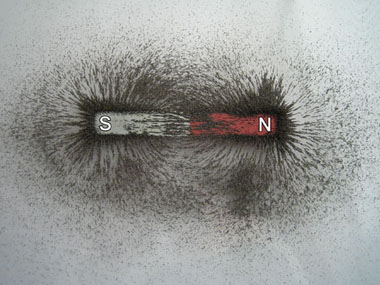
\includegraphics[width=0.5\textwidth]{unnamed.jpg}
    \caption{Representação de um imã e seus pólos. Ao redor, pó de ferro foi colocado para indicar o comportamento do magnetismo}
    \label{fig:ima}
\end{figure}

\section{Características principais}
\subsection{Indivisibilidade dos Pólos}
Quando falamos de imãs, sempre lembramos dos pólo norte e pólo sul e a primeira pergunta que temos é: \textbf{É possível separar os pólos de um imã?}

\textbf{A resposta é não. Qualquer material magnético tem que ter 2 pólos e por mais que você divida o material, cada pedaço sempre terá 2 pólos - um norte e um sul.}
\begin{figure}[H]
    \centering
    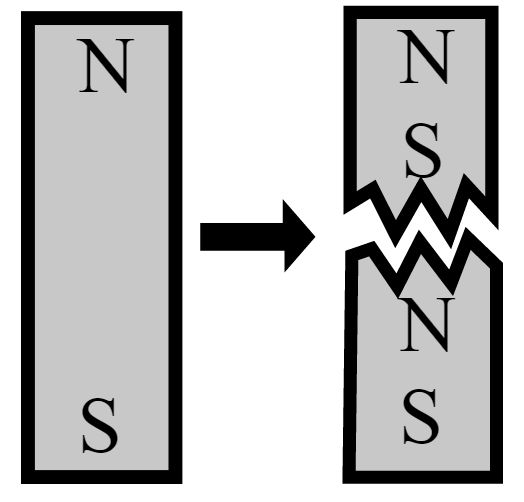
\includegraphics[width=0.2\textwidth]{57e42145ea362.jpg}
    \caption{Ilustração de como seria caso dividíssemos um imã em 2 partes e como os seus pólos se organizariam.}
    \label{fig:divisao_polo}
\end{figure}

\subsection{Atração e Repulsão}
Assim como na eletricidade, o magnetismo possui os fenômenos de atração e repulsão. Igual à eletricidade, \textbf{a atração ocorre entre os pólos opostos, enquanto a repulsão ocorre entre pólos iguais.} Ou seja, o Pólo Norte de um imã atraí o Pólo Sul de um outro imã, enquanto repel o Pólo Norte do outro imã.

\begin{figure}[H]
    \centering
    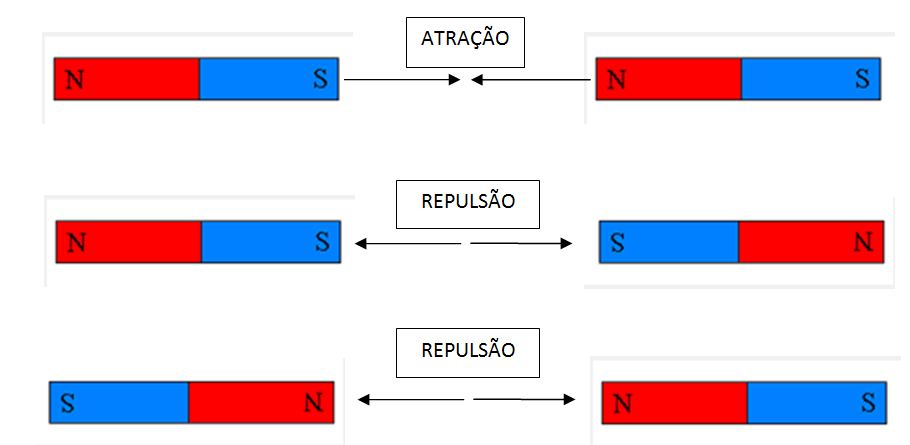
\includegraphics[width=0.8\textwidth]{mag4.png}
    \caption{Esquemas de atração e repulsão.}
    \label{fig:atracao}
\end{figure}

\subsection{Relação com os pólos da Terra}

A Terra gera um próprio magnetismo devido ao movimento de uma grande quantidade de ferro líquido no núcleo da Terra, veremos mais para frente como isso acontece. Esse magnetismo cria um campo magnético, veremos a seguir o que é isso, que sai do pólo sul da Terra e vai até o pólo norte. Porém, temos que tomar cuidado com a noção de pólos norte e sul:
\begin{align*}
\boxed{\begin{array}{c}
    &\text{\textbf{Pólo Norte da Terra}} \Longleftrightarrow \text{\textbf{Pólo Sul Magnético}}\\
    &\text{\textbf{Pólo Sul da Terra}} \Longleftrightarrow \text{\textbf{Pólo Norte Magnético}}
    \end{array}}
\end{align*}

\section{Campo Magnético ($\vec{B}$)}

A quantidade mais importante do magnetismo é o chamado \textbf{Campo Magnético. Ele é uma quantidade que se refere à concentração de magnetismo num ponto, ou seja, o quão atrativo/repulsivo magneticamente um objeto é, num ponto dado.}

O exemplo mais clássico de ilustração do campo magnético é o caso do campo produzido por um imã:

\begin{figure}[H]
    \centering
    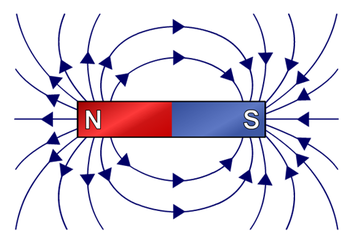
\includegraphics[width=0.6\textwidth]{main-qimg-410abffadd25e28bd5dfa66f0efb9e65.png}
    \caption{Ilustração do campo magnético produzido por um imã}
    \label{fig:magnetic_field}
\end{figure}

Uma questão importante: \textbf{O campo magnético sempre sai do pólo norte e chega no pólo sul.} A unidade do campo magnético é dada em \textbf{Tesla (T)}, em memória ao físico sérvio Nikola Tesla (1856-1943).

Com essa descrição, podemos, agora, embasar o conhecimento de porque pólos iguais se repelem e pólos iguais se atraem.
\begin{figure}[H]
     \centering
     \begin{subfigure}[b]{0.45\textwidth}
         \centering
         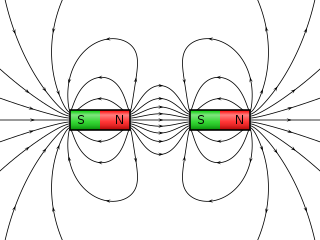
\includegraphics[width=\textwidth]{VFPt_cylindrical_magnets_attracting.svg.png}
         \caption{Esquema de atração entre imãs}
         \label{fig:attraction_mag_field}
     \end{subfigure}
     \hfill
     \begin{subfigure}[b]{0.45\textwidth}
         \centering
         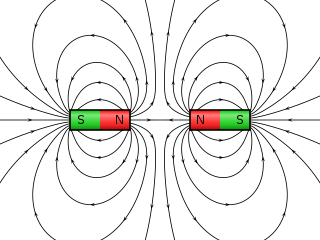
\includegraphics[width=\textwidth]{320px-VFPt_cylindrical_magnets_repelling.svg.png}
         \caption{Esquema de repulsão entre imãs}
         \label{fig:repulsion_mag_field}
     \end{subfigure}
\end{figure}

No caso da atração, as linhas do campo magnético estão mais juntas entre os imãs e nessa região, o magnetismo é bem forte. Além disso, as linhas se "atraem" entre si, fazendo a atração entre os imãs ser mais forte. 

Já no caso da repulsão, como os pólos nortes estão voltados um na frente do outro e o campo magnético sai do pólo norte, as linhas do campo tem em que encontrar um pólo sul. Com isso, essas linhas se empurram uma da outra, acontecendo a repulsão.

\section{Interação entre cargas elétricas e magnetismo}
Durante os estudos sobre o magnetismo, percebeu-se que as cargas elétricas, além de serem os agentes da eletricidade, também participavam de fenômenos magnéticos. Com isso, estudaram a forma como os campos magnéticos agiam nas cargas.

A primeira questão vista foi a \textbf{Força Magnética ($\vec{F}_{mag}$)} que é dada por:
\begin{equation}
    F_{mag} = q\,v\,B\,sen\,\theta
\end{equation}
\noindent em que 'q' é a carga que está no campo magnético, 'v' é a velocidade da carga, 'B' é o campo magnético agindo na carga e '$sen\,\theta$' é o ângulo feito \textbf{entre a velocidade e o campo magnético}.

Perceba que para a força ser nula ou a carga tem que estar parada ou a região onde ela está, não tem campo magnético.

Uma outra questão importante é a direção dessa força. A fórmula acima só nos dá a resposta escalar, mas sabemos que força, velocidade e o campo magnético são quantidades vetoriais. A direção da força é dada pela \textbf{Regra da Mão Esquerda:}
\begin{figure}[H]
    \centering
    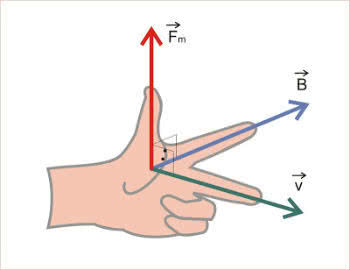
\includegraphics[width=0.6\textwidth]{regra_mao_esquerda.jpg}
    \caption{Ilustração da Regra da Mão Esquerda: \textbf{O polegar representa a direção da força ($\vec{F}_{mag}$), enquanto o dedo indicador representa a direção do campo magnético ($\vec{B}$) e o dedo médio representa a direção da velocidade ($\vec{v}$)}}
    \label{fig:my_label}
\end{figure}

\textbf{Essa regra vale para cargas positivas. Para cargas negativas, a direção da força é oposta ao resultado} (no caso da imagem acima, a força seria para baixo.)

Perceba que a força está numa direção diferente da direção da velocidade, então a carga irá fazer uma curva, na verdade, ela faz uma circunferência. 

Isso tudo permite a gente poder dizer que a \textbf{força magnética pode ser tratada como uma força centrípeta.} Vamos tratar somente o caso em que o ângulo entre a velocidade e o campo seja de 90$^\circ$, ou seja, $sen\,90^\circ =1$. Então:
\begin{equation}
    \begin{split}
        F_{mag} &= F_{cp}\\
        qvB &= \frac{mv^2}{R}\\
        R &= \frac{mv^2}{qvB} \implies \boxed{R = \frac{mv}{qB}}
    \end{split}
\end{equation}
\noindent em que $R$ é o raio da órbita que a carga faz, 'v' é a velocidade dela, 'm' é a massa da carga e 'B' é o valor do campo magnético.

O caso geral é quando a carga elétrica se movimenta um pouco na direção do campo elétrico e um pouco em outra direção. O que acontece no fundo, a carga vai começar a andar numa circunferência (por causa que uma parte da velocidade está numa direção diferente da direção do campo) enquanto anda para frente (porque a outra parte da velocidade está na mesma direção do campo magnético), fazendo o movimento helicoidal:
\begin{figure}[H]
    \centering
    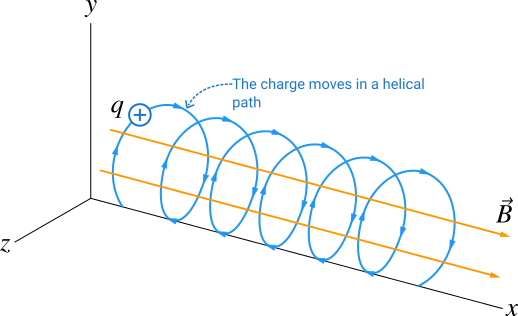
\includegraphics[width=0.5\textwidth]{charge-on-helix.png}
    \caption{Movimento Helicoidal de uma carga. A carga enquanto anda para frente, também roda como se estívesse num círculo.}
    \label{fig:my_label}
\end{figure}

Essa noção é usada para fazer armadilhas/prisão de cargas elétricas quando necessário, como em canhões de partículas, em que isso é usado para alinhar e focar as partículas. Outro uso é para fazer confinamento de cargas, como no meu trabalho em física de plasma para geração de energia.

\section{Eletrodinâmica - a relação entre Elétrica e Magnetismo}

Em 1831-32, o físico inglês Michael Faraday e o físico estadunidense Joseph Henry descobriram, de forma independente, os primeiros indícios da relação entre a eletricidade e magnetismo por meio da indução magnética.

A partir daí, junto com o trabalho teórico de Franz Neumann, é que se descobriu a chamada \textbf{Lei de Faraday}, que relacionava o magnetismo como causa de um efeito elétrico.

Em 1825, o físico francês Jean-Marie Àmpere descobriu que o campo magnético é gerado a partir de uma corrente elétrica não-nula. Nesse caso, o magnetismo é a consequência da eletricidade.

Aparentemente, temos um problema: uma lei diz que a eletricidade é a causa, enquanto a outra diz que é a consquência. \textbf{Mas, só em 1873, o físico inglês James Clerk Maxwell entendeu que a eletricidade e o magnetismo são 2 fenômenos interligados. Não há eletricidade sem magnetismo e vice-versa}, como 2 lados de uma mesma moeda. Daí nasce o nome da matéria: \textbf{Eletromagnetismo} ou \textbf{Eletrodinâmica}.

\subsection{Fluxo magnético e indução magnética - Lei de Faraday}

Uma outra quantidade magnética importante é chamada de \textbf{Fluxo magnético}:
\begin{equation}
    \Phi_m = B\,A\,\cos\theta
\end{equation}
\noindent em que 'B' é o valor do campo elétrico, 'A' é a área por onde o campo magnético está atravessando e '$\cos\theta$' é o ângulo entre a direção do campo magnético e a direção normal da área (veja abaixo para ficar mais claro)
\begin{figure}[H]
    \centering
    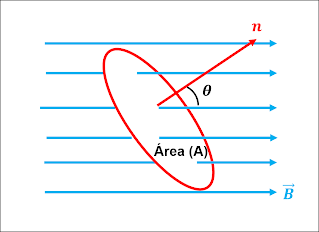
\includegraphics[width=0.5\textwidth]{indução 1.png}
    \caption{Esquema do fluxo magnético - o vetor em vermelho '$\vec{n}$' é o vetor normal, ele faz 90$^\circ$ com a área}
    \label{fig:my_label}
\end{figure}

Com essa quantidade, Michael Faraday percebeu que: \textbf{Se o fluxo magnético, que passa por uma área qualquer, variasse, uma f.e.m. (força eletromotriz) seria induzida de forma que a corrigir esse ganho/perda de fluxo.}
\begin{figure}[H]
    \centering
    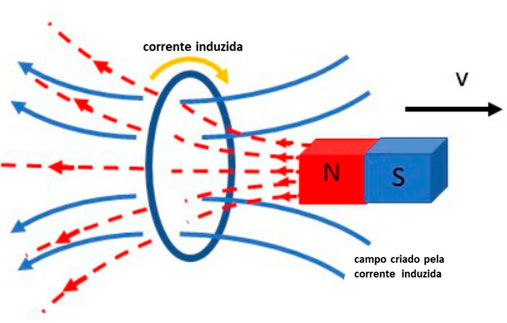
\includegraphics[width=0.5\textwidth]{corrente-induzida02.jpg}
    \caption{Ilustração da Lei de Lenz}
    \label{fig:lei_de_lenz}
\end{figure}

Para completar essa lei, uma outra foi descoberta pelo físico russo Emil Lenz. Essa outra lei foi chamada de Lei de Lenz que diz: \textbf{A direção da corrente elétrica induzida por um campo magnético externo é de forma que o campo magnético gerado pela corrente se oponha a mudança do campo magnético externo.} \footnote{é meio abstrato, eu sei, mas é a forma mais simples que eu consigo explicar.}

Com essas 2 leis, podemos formular a Lei de Faraday:
\begin{equation}
    \epsilon = - \frac{\Delta \Phi_m}{\Delta t} 
\end{equation}
\noindent em que '$\epsilon$' é a força eletromotriz (f.e.m.) e $\frac{\Delta \Phi_m}{\Delta t} = \frac{(\phi_m)_2 -(\phi_m)_1}{t_2 - t_1}$ é a variação do fluxo magnético dividido pelo tempo que levou a variação.


\subsection{Fórmulas dos campos magnéticos gerados por uma corrente}
\begin{enumerate}
    \item \textbf{Campo magnético gerado por uma corrente num fio retilíneo}:
    \begin{equation}
        B = \frac{\mu\,i}{2\pi\,R}
    \end{equation}
    \noindent em que $\mu$ é uma constante chamada '\textbf{permissividade magnética do vácuo}', 'i' é a corrente que passa no fio e 'R' é a distância do ponto de medição até o fio.
    
    \item \textbf{Campo magnético gerado por uma corrente numa espira (fio fechado em forma de circunferência)}:
    \begin{equation}
        B = \frac{\mu\,i}{2R}
    \end{equation}
    \noindent em que $\mu$ é uma constante chamada \textbf{constante de permissividade do vácuo}, 'i' é o valor da corrente que passa na espira, e 'R' é o raio da espira.
    
    \item \textbf{Campo magnético gerado por uma corrente passando num solenóide:}
    \begin{equation}
        B = \frac{\mu\,i\,n}{l}
    \end{equation}
    \noindent em que '$\mu$' é a constante chamada 'permeabilidade magnética do vácuo', 'i' é a corrente que passa no solenóide, 'n' é o número de voltas que o solenóide tem e 'l' é o comprimento dele.
\end{enumerate}

\begin{figure}[H]
     \centering
     \begin{subfigure}[b]{0.3\textwidth}
     \centering
         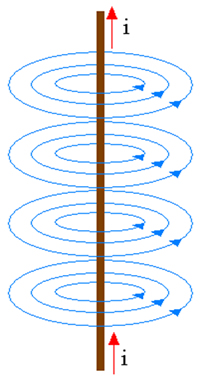
\includegraphics[width=\textwidth]{fio.jpg}
         \caption{Ilustração de um fio retilíneo e o campo magnético gerado por ele}
         \label{fig:fio}
     \end{subfigure}
     \hfill
     \begin{subfigure}[b]{0.3\textwidth}
         \centering
         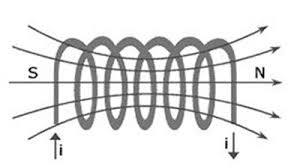
\includegraphics[width=\textwidth]{solenoide.jpg}
         \caption{Ilustração de um solenóide e o campo magnético gerado por ele}
         \label{fig:solenoide}
     \end{subfigure}
     \hfill
     \begin{subfigure}[b]{0.3\textwidth}
         \centering
         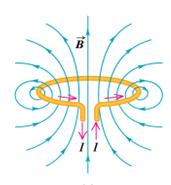
\includegraphics[width=\textwidth]{espira.jpg}
         \caption{Esquema de uma espira e o campo magnético gerado por ela}
         \label{fig:espira}
     \end{subfigure}
\end{figure}

O mais interessante do solenóide é que, em seu interior, \textbf{o campo magnético gerado é uniforme e constante.}

Por fim, para saber a direção do campo magnético gerado por uma espira, solenoide ou fio, temos a \textbf{Regra da Manivela ou a Regra da Mão Direita}:
\begin{figure}[H]
    \centering
    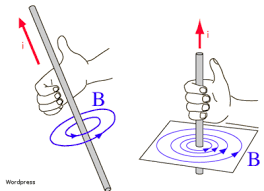
\includegraphics[width=0.4\textwidth]{regra_manivela.png}
    \caption{Ilustração da Regra da Manivela - a direção do dedão aponta a direção da corrente e o movimento dos outros dedos mostra como se comporta o campo magnético}
    \label{fig:my_label}
\end{figure}
\end{document}
